\section{Processing of Two Subject-Verb Dependencies in NLMs and Humans}
The core mechanism to carry agreement information across long-range dependencies in NLMs involves a very small number of units--one (Italian) or two (English). This mechanism was shown to robustly process sentences having a single long-range dependency. We next ask: given that the long-range agreement mechanism is sparse, and can thus only encode a single number feature at a time, how will the NLM process \emph{two} long-range dependencies that are active at once?

Two simultaneously active long-range dependencies occur in various constructions, such as center-embedded nested dependencies, a prototypical example of recursion. In nested dependencies, once the long-range agreement mechanism is engaged in tracking the main dependency, there may be no more suitable units available to process the \textit{embedded} agreement. For example, in the sentence ``The \textbf{boy} that the \textit{farmer} near the \underline{fathers} \textit{watches} \textbf{knows} the daughters'', there are two grammatical numbers that need to be carried across a long-range dependency: (1) that of the main subject `boy', and (2) that of the embedded subject `farmer'. Once the NLM  encounters the main subject, its grammatical number can be stored through the long-range agreement mechanism up to the main verb `knows'. However, during this period, since the mechanism is already taken up, once the embedded subject `farmer' is presented to the network, there is no robust way to encode and carry its number up to the embedded verb `watches'. The NLM is thus predicted to fail to process the embedded dependency in nested structures.

We emphasize two conditions for this predicted failure:
\begin{itemize}
	\item The two dependencies are \textit{simultaneously} active at some point: if this is not the case, i.e., the dependencies are successive (e.g., ``The \textbf{boy} near the \underline{cars} \textbf{says} that the \textit{farmer} near the \underline{fathers} \textit{watches} the daughters''), the long-range mechanism can first complete processing the first dependency, and then reset before encoding the next one. 

    \item Both dependencies are \textit{long-range}: in the case
          of a short-range dependency nested within a long-range one
          (e.g., ``The \textbf{boy} that the \textit{farmer}
          \textit{watches} \textbf{knows} the daughters''), the
          embedded short-range dependency can still be processed by
          the short-range units we described above, although possibly in a less robust way compared to the main dependency. 
\end{itemize}

We next present the experimental design we used to confirm these predictions about the NLM, as well as to test whether they also extend to human subjects, which would suggest that the agreement processing system of the latter bears similarities to the one we uncovered in NLMs.

\subsection{Experimental Design}
To test the hypothesis that the sparsity of the long-range mechanism can lead to a significant processing difficulty at the embedded dependency, we create a two-by-two design that manipulates the above two conditions: (1) whether the two dependencies are \textit{successive} or \textit{nested}, and (2) whether the embedded dependency is \textit{short} or \textit{long} range. 
Figure \ref{fig:design} describes the resulting four NA-tasks: Short-Successive, Long-Successive, Short-Nested and Long-Nested (`Short' and `Long' therefore refer to the length of the embedded dependency only). 

The successive tasks serve as control. They minimally differ from the nested ones up to the embedded verb, by only a single word (`dice' (`says') in Figure \ref{fig:design}). Note also that tasks that have a long embedded dependency have a third noun, which functions as a possible attractor, inside the embedded dependency. We will refer to this most-deeply embedded noun as the attractor, although the subjects of the main and nested clauses can also act as attractors on each others' verbs.

For each NA-task, we generate various \textit{conditions} by varying the number of the main and embedded subject noun, and that of the attractor. Short-Successive and Short-Nested have each four conditions corresponding to the possible assignments of number to the main and embedded subjects - SS, SP, PS and PP. Similarly, Long-Successive and Long-Nested have eight conditions, based on the possible numbers of the main, embedded subject and attractor - SSS, SSP, SPS, etc. In what follows, by \textit{congruent subjects} we refer to conditions in which the main and embedded subjects share grammatical number (SS, PP, SSS, SSP, PPS and PPP), and by \textit{incongruent subjects} to the rest (SP, PS, SPS, etc.). By \textit{congruent attractor}, we refer to conditions in which the embedded subject and the third noun share grammatical number (SSS, SPP, PSS and PPP), and by \textit{incongruent attractor} to conditions in which they differ (SSP, SPS, PSP, PPS) (Materials and Methods).

Several studies reported markedness effects in agreement, whereby humans make more errors when the grammatical number of the attractor is plural. This effect was reported in several languages and in both comprehension and production (\textit{English}: \citet{Bock:Miller:1991, eberhard1997marked, wagers2009agreement}; \textit{Italian}: \citet{vigliocco1995constructing}; \textit{Spanish}: \citet{bock2012number, lago2015agreement}; \textit{French}: \citet{franck2002subject}; \textit{Russian}: \citet{lorimor2008agreement}). Since we use error rates as an index of processing difficulties across various conditions, we strove to increase their overall signal. Therefore, we first present all analyses on contrasts with a plural attractor.
Results for the full set of conditions, with both singular and plural attractors, are reported subsequently.

Table \ref{tbl:predictions} summarizes our predictions for each task and structure, while ignoring for now, for ease of presentation, differences among specific conditions. 
For Short- and Long-Successive, no significant processing difficulties are predicted, since the long-range mechanism can encode the main and nested grammatical numbers sequentially. 
For Short- and Long-Nested, the long-range mechanism is predicted to successfully process the main dependency and therefore no significant difficulties are predicted on the main verb (beyond the relative difficulty to process center-embeddings reported for both humans \citep{traxler2002processing} and NLMs \citep{marvin2018targeted}). In contrast, the embedded dependency in Short-Nested cannot rely on the long-range agreement mechanism, as it is recruited by the main dependency. Consequently, the processing of the embedded dependency can only rely on short-range mechanisms, which might not be as robust as the long-range ones. We are thus agnostic about success in this case. Finally, in Long-Nested, the performance on the embedded verb is predicted to be significantly low, given that the long-range mechanism can process only a single agreement, as described above.

\begin{figure}[ht]
    \centering
    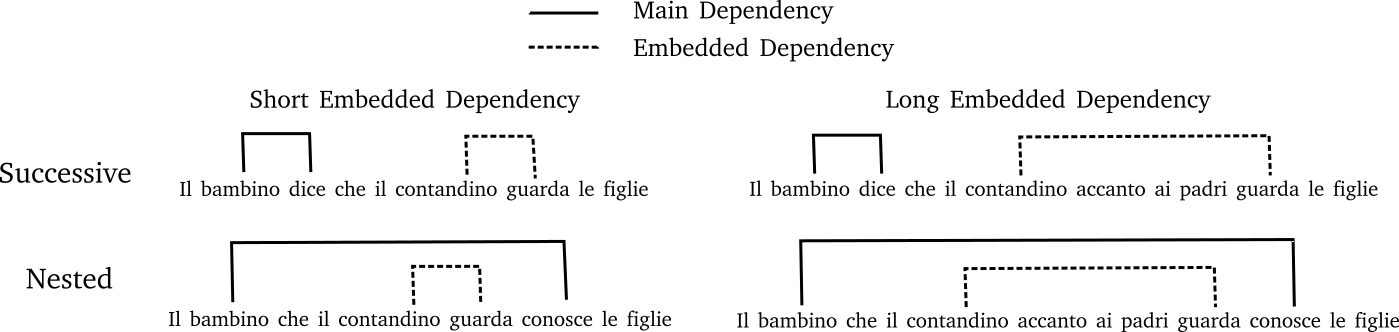
\includegraphics[width=\textwidth]{figures/design.png}
    \caption{\textbf{A full-factorial design for two subject-verb dependencies}. Human subjects and Neural Language Models were presented with sentences from four different syntactic structures, which all have two subject-verb dependencies: a main dependency (continuous lines) and an embedded dependency (dashed). The first factor of the design determines whether the two dependencies are \textit{successive} (top structures) or \textit{nested} (bottom), depending on whether the structure has a sentential complement or an object-extracted relative clause, respectively. The second factor determines whether the embedded dependency is \textit{short} (left side) or \textit{long} (right). We refer to the four resulting structures as: Short-Successive, Long-Successive, Short-Nested, Short-Long.}
    \label{fig:design}
\end{figure}
\begin{figure}[ht]
    \centering
    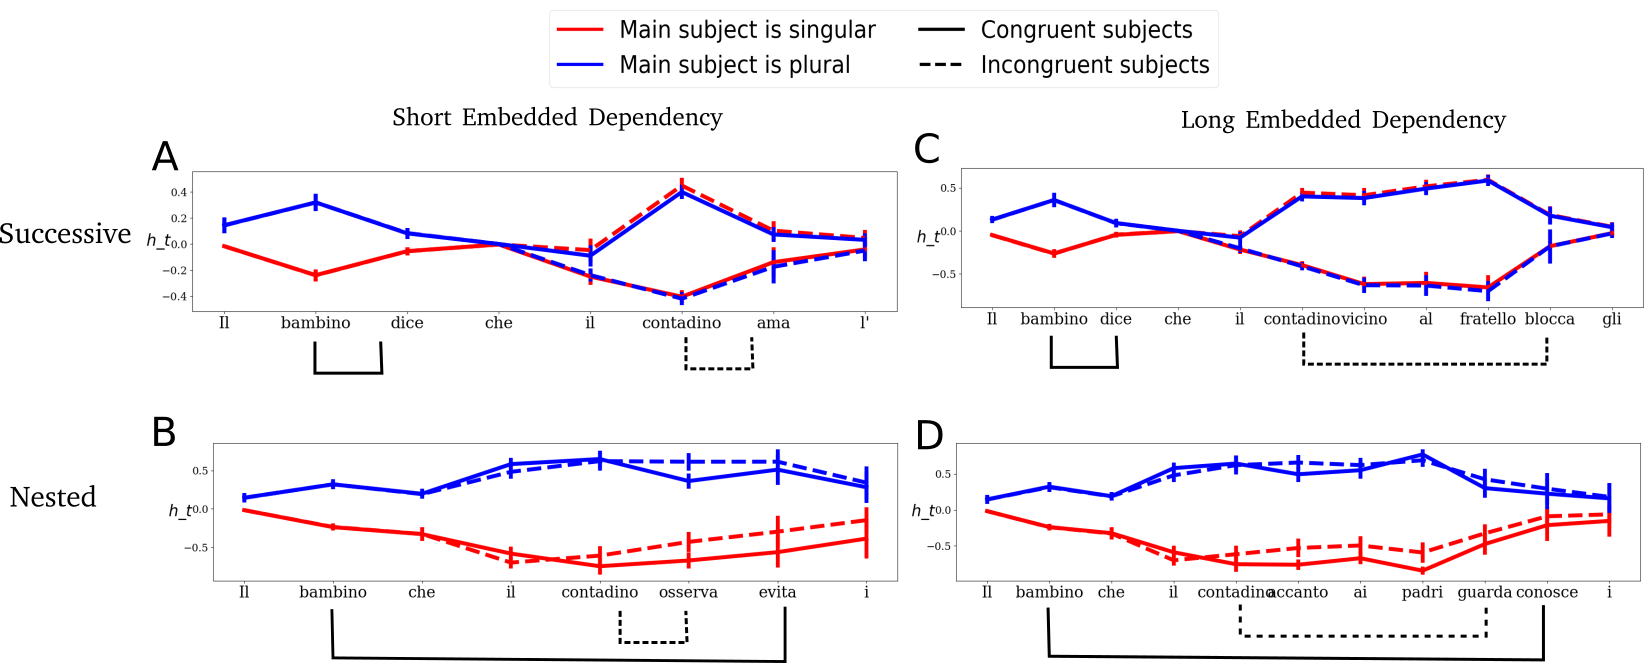
\includegraphics[width=\textwidth]{figures/model_activations.png}
    \caption{\textbf{Dynamics of the hidden activation of the number unit during the processing of two subject-verb dependencies.} Number-unit activity is presented for the four structures in the design: Short-Successive (panel A), Long-Successive (B), Short-Nested (C) and Long-Nested (D). For each structure, results are presented for four cases, corresponding to whether the main subject of the sentence is singular (red curves) or plural (blue), and to whether the main and embedded subjects have the same grammatical number (congruent; continuous lines) or not (incongruent; dashed lines).}
    \label{fig:2by2_dynamics}
\end{figure}

\begin{center}
\begin{table}
\centering
\begin{tabular}{|P{3.5cm}||P{3.5cm}|P{3.5cm}|}
    \hline
    \B Sentence Type & \B Main Verb & \B Embedded Verb \\
    \hline
    Successive-Short & V  & V \\
    \hline
    Successive-Long & V & V \\
    \hline
    Nested-Short & V & - \\
    \hline
    Nested-Long & V & X \\
    \hline
\end{tabular}
\caption{A summary of the predictions of model performance on successive and nested dependencies based on the sparsity of the long-range mechanism. 'V' and 'X' represent high and low predicted performance on the agreement task, respectively. Due to possible compensation mechanisms carried by the short-range number units, we make no precise predictions regarding performance on the embedded verb of Nested-Short.}
\label{tbl:predictions}
\end{table}
\end{center}


\subsection{Results for the Italian NLM}
\subsubsection{The Number Unit Shows Sequential Processing of Two Successive Dependencies and Robust Encoding of the Main Dependency in Nested Constructions}
We first simulate NLM dynamics for all NA-tasks and conditions, by presenting all sentences from each condition to the NLM (Materials and Methods). Figure \ref{fig:2by2_dynamics} presents hidden-state dynamics of the long-range number unit during the processing of all conditions from the four NA-tasks. We note that, consistent with results on a single dependency, the grammatical number of the main subject is encoded with the same polarity as found in the Noun-PP task - positive for plural (blue) and negative for singular (red). Second, in successive NA-tasks, the activation of the number unit returns to baseline after encountering the main verb (`dice'), and then rises back once the embedded subject is encountered. This shows that the number unit can sequentially encode two grammatical numbers in two successive dependencies, also when the two numbers are opposite. In particular, note that in Long-Successive, the grammatical number of the embedded subject is robustly carried across the attractor (`fratello') in the incongruent conditions (dashed lines). Finally, in both Short- and Long-Nested, the grammatical number of the main subject is robustly carried across the main dependency up to the main verb (`evita') \YL{fix xticklabels}, and in particular, across the embedded subject and verb that carry an opposite number in some conditions (dashed lines).

\textbf{M: The full-condition results seem to just cause information overload, and I would move them to an appendix.}

\textbf{M: Can we say $z$ and $p$ instead of $z-value$ and $p-value$? Besides making the blocks of quantitative results more readable, that would avoid the current ugly rendering with space before and after a long dash, which I invariably read as ``z minus value'', ``p minus value''.}

\subsubsection{NLM Performance on Successive Dependencies}
Since no significant processing difficulty is predicted in the successive tasks, we conduct the experiments on the embedded agreement only, which is expected to be the more difficult one. 
This allows us to reduce experimental duration in the parallel study with human participants. Also, to facilitate the interpretation of the results, we group conditions by whether the main and embedded subjects are congruent or not.

Figure \ref{fig:error_rates_plural_subject}A presents the resulting NLM error rates (Figure \ref{fig:error_rates_all_conditions} further provides the full error-rate distribution across all conditions). Several effects are observed in the results: 

\begin{itemize}
    \item \textbf{Near perfect performance on all conditions}: Overall, for both Short- and Long-Successive, the performance of the NLM was found to be almost error free, with slightly more errors in the Long-Successive case ($z-value=26.3, p-value<0.001$)
    \item \textbf{Subject-congruence effect}: We next tested for a \textit{subject-congruence effect}, i.e., whether incongruent subjects elicited more errors compared to congruent ones. We found a significant subject-congruence effect in both Short- and Long-Successive (Short-Nested: $z-value=5.4, p-value<0.001$; Long-Nested: $z-value=6.4, p-value<0.001$). Note that the variance of the network is very low, which renders this effect significant, although the error-rate is near zero in both congruent and incongruent cases.
\end{itemize}
 
 \begin{figure}[ht]
    \centering
    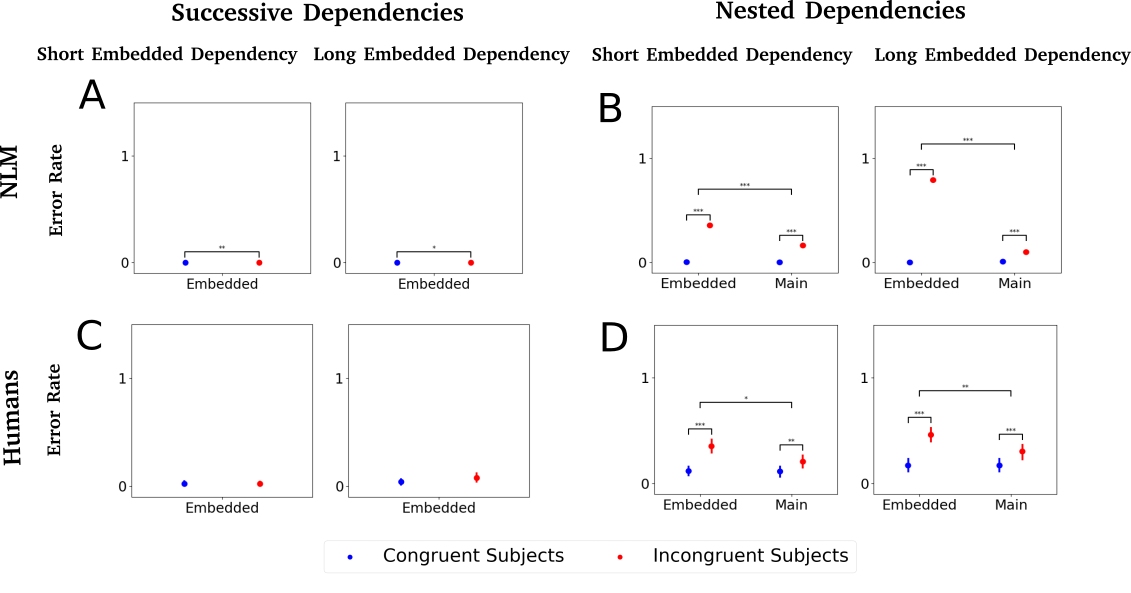
\includegraphics[width=16cm]{figures/error_rates_plural_subject.png}
    \caption{\textbf{Error rates for all four NA-tasks:} collected from the NLM (panels A \& B) and human subjects (C \& D). Blue and red correspond to whether the main and embedded subjects agree on number (congruent subjects) or not (incongruent), respectively. Error bars represent standard error of the mean across all trials.}
    \label{fig:error_rates_plural_subject}
\end{figure}

\begin{figure}[ht]
    \centering
    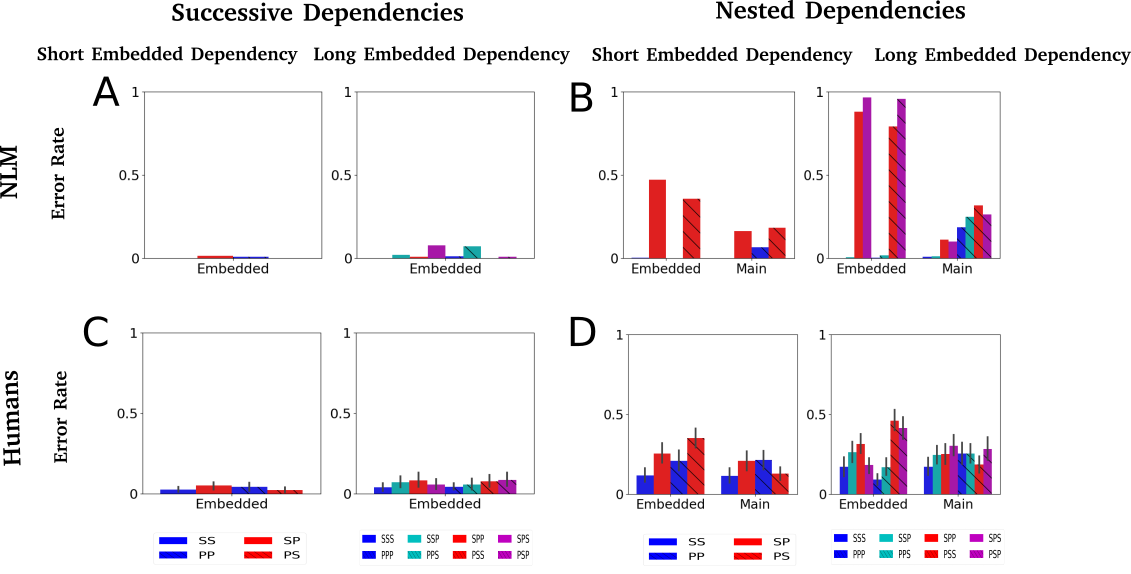
\includegraphics[width=16cm]{figures/error_rates_all_conditions.png}
    \caption{\textbf{Error rates for all conditions:} collected from the NLM (panels A \& B) and human subjects (C \& D). Bluish and reddish colors correspond to whether the main and embedded subjects agree on number (congruent subjects) or not (incongruent), respectively. Secondary colors (cyan or magenta) represent the presence of a nested attractor carrying an opposite grammatical number. Bars with stripes correspond to conditions in which the main subject is plural. Error bars represent standard error of the mean across all trials.}
    \label{fig:error_rates_all_conditions}
\end{figure}
 
\subsubsection{NLM Performance on Nested Dependencies}
Figure \ref{fig:error_rates_plural_subject}B presents the corresponding error-rates in the case of nested dependencies (Figure \ref{fig:error_rates_all_conditions} further provides the full error-rate distribution across all conditions). Several effects are observed in the results:

\begin{itemize}
    \item \textbf{Incongruent conditions elicit more errors}: a significant subject-congruence effect was found on both the embedded and main verbs, in both Short- and Long-Nested (Short-Nested main: $z-value=93.1, p-value<0.001$; Short-Nested embedded: $z-value=50.9, p-value<0.001$; Long-Nested main: $z-value=67.0, p-value<0.001$; Long-Nested embedded: $z-value=120.5, p-value<0.001$). In all cases, incongruent subjects elicited more errors compared to congruent subjects.
    \item \textbf{Processing of embedded verbs is more error-prone}: for both Short- and Long-Nested, a significant interaction was found between subject-congruence and verb-position (embedded/main), with a larger increase of error rate due to incongruent subjects on the embedded compared to the main verb (Short-Nested: $z-value=32.3, p-value<0.001$; Long-Nested: $z-value=84.2, p-value<0.001$).
    \item \textbf{A longer embedded dependency is more error prone}: for errors made on the embedded verb, we found a significant interaction between subject-congruence and the length of the embedded dependency (Short/Long-Nested), with a larger increase of error-rate due to incongruent subjects in Long-Nested ($z-value=7.4, p-value<0.001$).
\end{itemize}
 
\vspace{10pt}

\subsubsection{Discussion of NLM results}
Focusing on cases with incongruent subjects, the error patterns of the NLM are overall consistent with the predictions summarized in Table \ref{tbl:predictions}. First, successive dependencies are relatively easy for the model, and can be processed sequentially. This is consistent with the sequential encoding observed in the dynamics of the number unit (Figure \ref{fig:2by2_dynamics}), which shows a robust encoding of grammatical number of embedded subjects, also in the presence of an attractor. Second, the main dependency in both Short- and Long-Nested was successfully processed (i.e., significantly better than chance level), although with more overall errors compared to successive dependencies. Third, the NLM made an exceptionally large number of errors on the embedded verb in Long-Nested, as predicted by the sparsity of the long-range mechanism. This is prominent in the case of incongruent-subject, since only then the grammatical number of the main subject encoded in the long-range mechanism can interfere. Finally, the NLM made a relatively large number of errors on the embedded verb in Short-Nested but was significantly better than chance level ($error-rate = 0.5$; $p-calue < 0.001$). The reduced number of errors in Short- compared to Long-Nested is consistent with the findings about a less sophisticated short-range mechanism that can process the embedded dependency, compensating for the momentary recruitment of the long-range mechanism for the main one. 

\subsection{Results for Humans}
The previous section has shown that the NLM cannot robustly encode two long-range dependencies that are active at once. The NLM: (1) made more errors on the embedded verb in both Short- and Long-Nested, and (2) had an exceptionally high error rate in the latter case, when the embedded dependency was long range.

Suppose that a similarly sparse mechanism is also used by humans to carry number features through long-distance agreement structures. We derive the following predictions:
% \dnote{I'm a bit in doubt about this transition, for two reasons: 
% 1) This is quite an important point, currently it is put very lightly. I think it would be good to put a bit more stress on it.
% 2) It seems a bit now that these predictions are sort of re-derived. Should we not be more clear about the fact that this directly follows from what we observed in the LM? I know there is some explanation relating to the LM afterwards, but I would opt to make it clear from the beginning.
% }

\begin{itemize}
    \item \textbf{Prediction 1}: humans will make more agreement errors on the embedded compared to the main dependency in the incongruent conditions of Long-Nested. 
    \item \textbf{Prediction 2}: humans will make more errors on the incongruent conditions of the embedded verb when the embedded dependency is long- compared to short-range.
\end{itemize}

Prediction 1 derives from the robustness of the agreement mechanism in processing the main but not the embedded dependency, as was observed in the NLM performance. The prediction is particularly interesting because, structurally, the main dependency will always be longer-range than the embedded one. Note that we we don't make precise predictions regarding Short-Nested, due to possible short-range compensation mechanisms in humans. Prediction 2 derives from the sparsity of the agreement mechanism and the dramatic failure of the model to process the embedded dependency in Long- but not Short-Nested. 

We test these predictions by presenting Italian speakers with sentences from the same four NA-tasks in the design (Figure \ref{fig:design}; Methods and Materials). In what follows, we describe the resulting agreement-error patterns in humans and then compare them to those of the NLM.

\subsubsection{Human Performance on Successive Dependencies}
Figure \ref{fig:error_rates_plural_subject}C presents the resulting human error rates (Figure \ref{fig:error_rates_all_conditions} further provides the full error-rate distribution across all conditions). Several effects are observed in the results: 

\textbf{M: Small style point: I think that when ``error rate'' is used an independent noun (as opposed to modifier) it should have no dash. So, error-rate distribution, but: relatively low error rate. I adjusted some cases to match my usage, but perhaps I have not been systematic enough.}

\begin{itemize}
    \item \textbf{Relatively low error rate}: humans made relatively few errors on successive constructions, although significantly above zero. Note that, in comparison to the Italian NLM, humans have a higher error baseline, to which unrelated factors that are specific to humans may contribute, such as occasional lapses of attention.
    \item \textbf{No subject-congruence effect}: we found no significant subject-congruence effect in Short-Successive, and a marginally significant subject-congruence effect in Long-Successive ($z-value=1.834, p-value=0.06$).
\end{itemize}

\subsubsection{Human Performance on Nested Dependencies}
Figure \ref{fig:error_rates_plural_subject}D presents the resulting human error rates (Figure \ref{fig:error_rates_all_conditions} further provides the full error-rate distribution across all conditions). Several effects are observed in the results:

\begin{itemize}
    \item \textbf{Subject-congruence effect on embedded and main verbs}: for both main and embedded verbs in both Short- and Long-Nested, incongruent subjects elicited more errors--a significant subject-congruence effect was found in all cases (Short-Nested main: $z-value=2.970, p-value=0.003$; Short-Nested embedded: $z-value=6.411, p-value<0.001$; Long-Nested main $z-value=3.630, p-value<0.001$; Long-Nested embedded: $z-value=7.274, p-value<0.001$).
    \item \textbf{Processing of embedded verbs is more error-prone}: for both Short- and Long-Nested, the increase in error rate due to incongruent subjects was larger for embedded compared to main verbs. A significant interaction was found between subject congruence and verb position in both cases (Short-Nested: $z-value=2.277, p-value = 0.02$, Long-Nested: $z-value=2.634, p-value = 0.008$).
    \item \textbf{A longer embedded dependency is not significantly more error prone}: for embedded verbs, the increase in error-rate due to incongruent subjects was comparable when the embedded long-range dependency was compared to the short one. No significant interaction was found between subject-congruence and length of the embedded dependency (Short- vs. Long-Nested).
\end{itemize}


\subsection{Markedness effect in humans and NLM}
\textbf{M: What is the reason to put this in the main? The issue of whether plural is also a marked feature for NLMs is interesting (for example, to test theories that markedness is a function of statistical trends that should also be picked up by language models). However, in the context of our discussion, I find it quite distracting. I would vote for moving it entirely to the appendix (together with the full-results analyses above).}

Finally, we tested for markedness effects in both humans and the NLM.
For each verb in each of the four NA-task, we fitted a logistic-regression model with subject-congruence and grammatical number of the intervening subject as variables. Note that, while for embedded verbs the intervening subject is the main subject, for main verbs, the intervening subject is the embedded subject. In the case of Long-Successive and Long-Nested, we also included congruence of the embedded subject and the nested attractor as a variable in the regression model. 

In humans, we found significant main effects for the grammatical number of the intervening subject in the following cases: embedded and main verbs in Short- and Long-Nested (Short-Nested: $\beta^{embedded}=0.47; p-value<0.05$ and $\beta^{main}=0.56; p-value<0.05$; Long-Nested: $\beta^{embedded}=0.67; p-value<0.001$ and $\beta^{main}=0.47; p-value<0.05$; positive $\beta$ indicates more errors due to intervention of a plural number). In Long-Nested, we further found an interaction between subject-congruence and the grammatical number of the intervening attractor ($\beta^{interaction}=1.4173; p-value<0.001$). In contrast, in the NLM, an intervening plural noun did not generate more errors compared to singular. In several cases, the effect was reversed, i.e., an intervening singular noun caused more errors - Table S1\ref{} summarizes all effects found in both humans and the NLM. 


\subsubsection{Discussion of human results}
Overall, successive dependencies were, as expected, relatively easy for humans compared to nested ones. 
The subject-congruence effect was not found, or was marginally significant, which is consistent with sequential processing of grammatical number in NLMs. The results confirm \textit{Prediction 1}--the main dependency in both Short- and Long-Nested was less error prone than the embedded one, as was confirmed by a significant interaction between subject-congruence and verb position. However, although humans made more errors on the embedded dependency when it was long range, we did not find a significant interaction between subject-congruence and the length of the embedded dependency. Prediction 2 was therefore not confirmed by the results.